\documentclass[10pt]{article}
\usepackage[utf8]{inputenc}
\usepackage[T1]{fontenc}
\usepackage{amsmath}
\usepackage{amsfonts}
\usepackage{amssymb}
\usepackage[version=4]{mhchem}
\usepackage{stmaryrd}
\usepackage{graphicx}
\usepackage[export]{adjustbox}
\graphicspath{ {./images/} }
\usepackage{caption}

%New command to display footnote whose markers will always be hidden
\let\svthefootnote\thefootnote
\newcommand\blfootnotetext[1]{%
  \let\thefootnote\relax\footnote{#1}%
  \addtocounter{footnote}{-1}%
  \let\thefootnote\svthefootnote%
}

%Overriding the \footnotetext command to hide the marker if its value is `0`
\let\svfootnotetext\footnotetext
\renewcommand\footnotetext[2][?]{%
  \if\relax#1\relax%
    \ifnum\value{footnote}=0\blfootnotetext{#2}\else\svfootnotetext{#2}\fi%
  \else%
    \if?#1\ifnum\value{footnote}=0\blfootnotetext{#2}\else\svfootnotetext{#2}\fi%
    \else\svfootnotetext[#1]{#2}\fi%
  \fi
}

\begin{document}

\section*{8 Ring of a planet (20 Points)}
We are given a flat disk of mass M with inner radius $r$ and the outer radius $R$.\\
(a) A point mass $m$ is located on the symmetry axis of the disk at a distance $x$ from the plane of the disk (We assume throughout that mass $m$ stays on the symmetry axis, and is free to move in the vertical direction.). What is the gravitational force exerted on the point mass?

\begin{figure}[h]
\begin{center}
  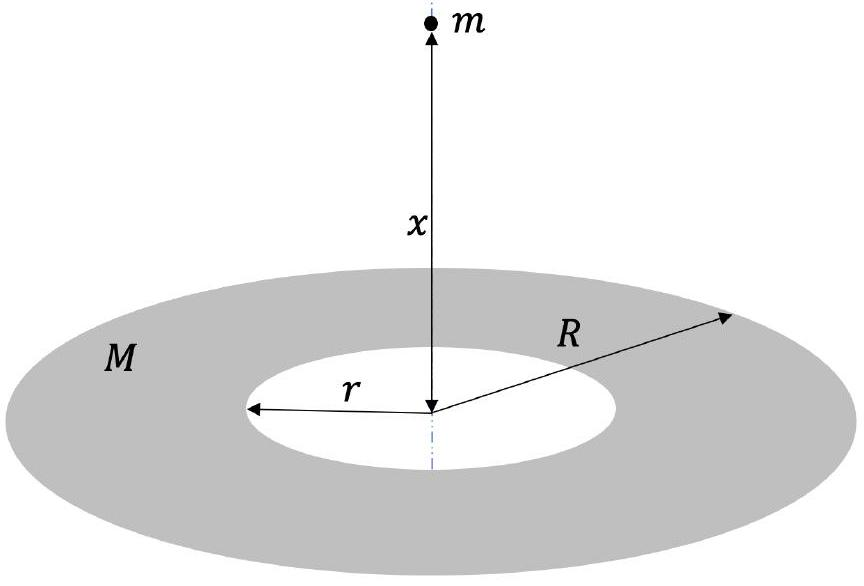
\includegraphics[width=\textwidth]{2025_09_11_6312450c103d6a7e5736g-05(1)}
\captionsetup{labelformat=empty}
\caption{Figure 2: Flat disk around a point mass}
\end{center}
\end{figure}

Hint 1: You may denote surface density by the symbol $\sigma$ and calculate force exerted by a small surface element $\Delta S$ subtending a solid angle $\Delta \Omega$ with $m$\\
Hint 2: The area cut by cone with opening angle $2 \theta$ on a sphere of radius $R$ :

$$
S=2 \pi R^{2}(1-\cos (\theta))
$$

\begin{figure}[h]
\begin{center}
  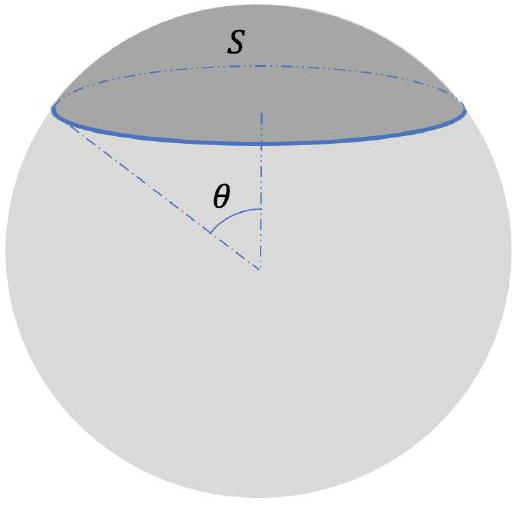
\includegraphics[width=\textwidth]{2025_09_11_6312450c103d6a7e5736g-05}
\captionsetup{labelformat=empty}
\caption{Figure 3: Area cut by a cone on a sphere}
\end{center}
\end{figure}

(b) what will be the frequency of the small oscillations of the system $(x \ll r)$.


\end{document}